\begin{enumerate}[label=\thesection.\arabic*,ref=\thesection.\theenumi]
\numberwithin{equation}{enumi}
\numberwithin{figure}{enumi}
\numberwithin{table}{enumi}
\item 
\label{chapters/9/10/4/1}
\iffalse
\documentclass[12pt]{article}
\usepackage{graphicx}
\usepackage{amsmath}
\usepackage{mathtools}
\usepackage{gensymb}

\newcommand{\mydet}[1]{\ensuremath{\begin{vmatrix}#1\end{vmatrix}}}
\providecommand{\brak}[1]{\ensuremath{\left(#1\right)}}
\providecommand{\norm}[1]{\left\lVert#1\right\rVert}
\newcommand{\solution}{\noindent \textbf{Solution: }}
\newcommand{\myvec}[1]{\ensuremath{\begin{pmatrix}#1\end{pmatrix}}}
\let\vec\mathbf

\begin{document}
\begin{center}
\textbf\large{CHAPTER-11 \\ CIRCLES}

\end{center}
\section*{Excercise 11.1}

Q4.Find the equation of the circle with centre $(1,1)$ and radius $\sqrt{2}$.

\solution
\fi
Given
\begin{align}
	\vec{c} &= \myvec{1\\1} \text{ and } r = \sqrt{2},
	\\
	\vec{u}&=\vec{-c}
	 = \myvec{-1\\-1}\\
	 \\
	f &= \norm{\vec{u}}^2 - r^2
	  =0	
\end{align}
Thus, the equation of circle is 
\begin{align}
	\norm{\vec{x}}^2 -2\myvec{1&1}\vec{x} = 0       		       
\end{align}	
See Fig. 
\ref{fig:chapters/11/11/1/4/Fig1}.
\begin{figure}[!h]
	\begin{center} 
	  \includegraphics[width=\columnwidth]{chapters/11/11/1/4/figs/circ.png}
	\end{center}
\caption{}
\label{fig:chapters/11/11/1/4/Fig1}
\end{figure}

\item If two equal chords of a circle intersect within the circle, prove 
that the segments of one chord are equal to corresponding segments of the other 
chord.
\label{chapters/9/10/4/2}
\\
\solution 
\iffalse
\documentclass[10pt]{article}
       \usepackage[latin1]{inputenc}
       \usepackage{fullpage}
       \usepackage{color}
       \usepackage{array}
       \usepackage{longtable}
       \usepackage{calc}
       \usepackage{multirow}
       \usepackage{hhline}
       \usepackage{ifthen}
\usepackage{graphicx}
\def\inputGnumericTable{}
\usepackage[none]{hyphenat}
\usepackage{graphicx}
\usepackage{listings}
\usepackage[english]{babel}
\usepackage{graphicx}
\usepackage{caption} 
\usepackage{booktabs}
\usepackage{gensymb}
\usepackage{array}
\usepackage{amssymb} % for \because
\usepackage{amsmath}   % for having text in math mode
\usepackage{extarrows} % for Row operations arrows
\usepackage{listings}
\lstset{
  frame=single,
  breaklines=true
}
\usepackage{hyperref}
%Following 2 lines were added to remove the blank page at the beginning
\usepackage{atbegshi}% http://ctan.org/pkg/atbegshi
\AtBeginDocument{\AtBeginShipoutNext{\AtBeginShipoutDiscard}}
%New macro definitions
\newcommand{\mydet}[1]{\ensuremath{\begin{vmatrix}#1\end{vmatrix}}}
\providecommand{\brak}[1]{\ensuremath{\left(#1\right)}}
\providecommand{\norm}[1]{\left\lVert#1\right\rVert}
\newcommand{\solution}{\noindent \textbf{Solution: }}
\newcommand{\myvec}[1]{\ensuremath{\begin{pmatrix}#1\end{pmatrix}}}
\providecommand{\abs}[1]{\left\vert#1\right\vert}
\let\vec\mathbf
\begin{document}
\begin{center}
\title{\textbf{Properties of Circle}}
\date{\vspace{-5ex}} %Not to print date automatically
\maketitle
\end{center}
\setcounter{page}{1}
\section{9$^{th}$ Maths - Chapter 10}
       This is Problem-2 from Exercise 10.4
\begin{enumerate}
\item If two equal chords of a circle intersect within the circle, prove that the segments of one chord are equal to corresponding segments of other chord.

\solution:
\fi
\begin{figure}[h!]
	\begin{center} 
	  \includegraphics[width=\columnwidth]{chapters/9/10/4/2/figs/c.png}
	\end{center}
\caption{Two equal chords intersecting in a circle}
\label{fig:chapters/9/10/4/2/Fig1}
\end{figure} 
See Table 
\ref{tab:chapters/9/10/4/2/}
for the input  parameters.
\begin{table}[h!]
	\begin{tabular}{|c|c|p{5cm}|}
\hline
\textbf{Symbol} & \textbf{Value} & \textbf{Description} \\
\hline
$\theta$ & $30\degree$ & $\angle{BAP} = \angle{BAQ}$ \\
\hline
$a$ & $9$ & $AB$ \\
\hline
$c$ & $8$ & $AQ$ \\
\hline
$\vec{e}_1$ & $\myvec{1\\0}$ & Basis vector \\
\hline
\end{tabular}

\caption{}
\label{tab:chapters/9/10/4/2/}
\end{table}
Consider
\begin{align}
\vec{P}=\myvec{\cos \theta_1\\\sin \theta_1},\,
\vec{Q}=\myvec{\cos \theta_2\\\sin \theta_2},\,
\vec{R}=\myvec{\cos \theta_3\\\sin \theta_3},\,
\vec{S}=\myvec{\cos \theta_4\\\sin \theta_4}
\label{eq:chapters/9/10/4/2/table1}
\end{align}
such that 
\begin{align}
	\vec{P}-\vec{Q}&=\myvec{\cos\theta_1-\cos\theta_2 \\ \sin \theta_1-\sin \theta_2}
	\\
	\implies \norm{\vec{P}-\vec{Q}}^2 &= 
	\brak{\cos \theta_1-\cos \theta_2}^2+\brak{\sin \theta_1-\sin \theta_2}^2=d^2\\
\end{align}
yielding
\begin{align}
	\brak{\frac{\theta_1-\theta_2}{2}}=\sin^{-1}\brak{\frac{d}{2}}.
	\end{align}
	Similarly, 
\begin{align}
\brak{\frac{\theta_3-\theta_4}{2}}=\sin^{-1}\brak{\frac{d}{2}}.
\end{align}
The equations of $PQ$ and $RS$ are obtained using 
\begin{align}
\vec{{n}_1^{\top}}\brak{\vec{x}-\vec{P}}&=0\\
\vec{{n}_2^{\top}}\brak{\vec{x}-\vec{R}}&=0
\end{align}
where 
\begin{align}
\vec{n}_1
&=\myvec{\sin \theta_1-\sin \theta_2\\\cos \theta_2-\cos \theta_1}\\
\vec{n}_2
&=\myvec{\sin \theta_3-\sin \theta_4\\\cos \theta_4-\cos \theta_3}
\end{align}
Substiuting numerical values, the 
point of intersection of lines $PQ,RS$ is 
\begin{align}
\vec{T}=\myvec{0.68341409\\-0.04288508}
\end{align}
Thus, 
\begin{align}
\norm{\vec{P}-\vec{T}}=
\norm{\vec{S}-\vec{T}}&=0.5727
\end{align}

\item If a line intersects two concentric circles (circles
with the same centre) with centre $\vec{O}$ at $\vec{A}$, $\vec{B}$, $\vec{C}$ and $\vec{D}$, prove that $AB = CD$.
		\label{chapters/9/10/4/4/}
\\
\solution 
\iffalse
\documentclass[12pt]{article}
\usepackage{graphicx}
\usepackage{amsmath}
\usepackage{mathtools}
\usepackage{gensymb}

\newcommand{\mydet}[1]{\ensuremath{\begin{vmatrix}#1\end{vmatrix}}}
\providecommand{\brak}[1]{\ensuremath{\left(#1\right)}}
\providecommand{\norm}[1]{\left\lVert#1\right\rVert}
\newcommand{\solution}{\noindent \textbf{Solution: }}
\newcommand{\myvec}[1]{\ensuremath{\begin{pmatrix}#1\end{pmatrix}}}
\let\vec\mathbf

\begin{document}
\begin{center}
\textbf\large{CHAPTER-11 \\ CIRCLES}

\end{center}
\section*{Excercise 11.1}

Q4.Find the equation of the circle with centre $(1,1)$ and radius $\sqrt{2}$.

\solution
\fi
Given
\begin{align}
	\vec{c} &= \myvec{1\\1} \text{ and } r = \sqrt{2},
	\\
	\vec{u}&=\vec{-c}
	 = \myvec{-1\\-1}\\
	 \\
	f &= \norm{\vec{u}}^2 - r^2
	  =0	
\end{align}
Thus, the equation of circle is 
\begin{align}
	\norm{\vec{x}}^2 -2\myvec{1&1}\vec{x} = 0       		       
\end{align}	
See Fig. 
\ref{fig:chapters/11/11/1/4/Fig1}.
\begin{figure}[!h]
	\begin{center} 
	  \includegraphics[width=\columnwidth]{chapters/11/11/1/4/figs/circ.png}
	\end{center}
\caption{}
\label{fig:chapters/11/11/1/4/Fig1}
\end{figure}

\item If a line intersects two concentric circles (circles with the same 
centre) with centre $\vec{O}$ at $\vec{A}, \vec{B}, \vec{C}, \vec{D}$, prove 
that $AB = CD$ (see Fig. 
		\ref{fig:chapters/9/10/41} ).
\begin{figure}[!ht]
    \centering
    \includegraphics[width=\columnwidth]{chapters/9/10/4/figs/fig1.jpg}
    \caption{}
    \label{fig:chapters/9/10/41}
\end{figure}
\item Three girls Reshma, Salma and Mandip are playing a game by standing on 
a circle of radius 5m drawn in a park. Reshma throws a ball to Salma, Salma to 
Mandip, Mandip to Reshma. If the distance between Reshma and Salma and between 
Salma and Mandip is 6m each, what is the distance between Reshma and Mandip?
\\
\solution 
\iffalse
\documentclass[journal,12pt,twocolumn]{IEEEtran}
%
\usepackage{setspace}
\usepackage{gensymb}
%\doublespacing
\singlespacing

%\usepackage{graphicx}
%\usepackage{amssymb}
%\usepackage{relsize}
\usepackage[cmex10]{amsmath}
%\usepackage{amsthm}
%\interdisplaylinepenalty=2500
%\savesymbol{iint}
%\usepackage{txfonts}
%\restoresymbol{TXF}{iint}
%\usepackage{wasysym}
\usepackage{amsthm}
%\usepackage{iithtlc}
\usepackage{mathrsfs}
\usepackage{txfonts}
\usepackage{stfloats}
\usepackage{bm}
\usepackage{cite}
\usepackage{cases}
\usepackage{subfig}
%\usepackage{xtab}
\usepackage{longtable}
\usepackage{multirow}
%\usepackage{algorithm}
%\usepackage{algpseudocode}
\usepackage{enumitem}
\usepackage{mathtools}
\usepackage{steinmetz}
\usepackage{tikz}
\usepackage{circuitikz}
\usepackage{verbatim}
\usepackage{tfrupee}
\usepackage[breaklinks=true]{hyperref}
%\usepackage{stmaryrd}
\usepackage{tkz-euclide} % loads  TikZ and tkz-base
%\usetkzobj{all}
\usetikzlibrary{calc,math}
\usepackage{listings}
    \usepackage{color}                                            %%
    \usepackage{array}                                            %%
    \usepackage{longtable}                                        %%
    \usepackage{calc}                                             %%
    \usepackage{multirow}                                         %%
    \usepackage{hhline}                                           %%
    \usepackage{ifthen}                                           %%
  %optionally (for landscape tables embedded in another document): %%
    \usepackage{lscape}     
\usepackage{multicol}
\usepackage{chngcntr}
%\usepackage{enumerate}

%\usepackage{wasysym}
%\newcounter{MYtempeqncnt}
\DeclareMathOperator*{\Res}{Res}
%\renewcommand{\baselinestretch}{2}
\renewcommand\thesection{\arabic{section}}
\renewcommand\thesubsection{\thesection.\arabic{subsection}}
\renewcommand\thesubsubsection{\thesubsection.\arabic{subsubsection}}

\renewcommand\thesectiondis{\arabic{section}}
\renewcommand\thesubsectiondis{\thesectiondis.\arabic{subsection}}
\renewcommand\thesubsubsectiondis{\thesubsectiondis.\arabic{subsubsection}}

% correct bad hyphenation here
\hyphenation{op-tical net-works semi-conduc-tor}
\def\inputGnumericTable{}                                 %%

\lstset{
%language=C,
frame=single, 
breaklines=true,
columns=fullflexible
}
%\lstset{
%language=tex,
%frame=single, 
%breaklines=true
%}

\begin{document}
%


\newtheorem{theorem}{Theorem}[section]
\newtheorem{problem}{Problem}
\newtheorem{proposition}{Proposition}[section]
\newtheorem{lemma}{Lemma}[section]
\newtheorem{corollary}[theorem]{Corollary}
\newtheorem{example}{Example}[section]
\newtheorem{definition}[problem]{Definition}
%\newtheorem{thm}{Theorem}[section] 
%\newtheorem{defn}[thm]{Definition}
%\newtheorem{algorithm}{Algorithm}[section]
%\newtheorem{cor}{Corollary}
\newcommand{\BEQA}{\begin{eqnarray}}
\newcommand{\EEQA}{\end{eqnarray}}
\newcommand{\define}{\stackrel{\triangle}{=}}

\bibliographystyle{IEEEtran}
%\bibliographystyle{ieeetr}


\providecommand{\mbf}{\mathbf}
\providecommand{\pr}[1]{\ensuremath{\Pr\left(#1\right)}}
\providecommand{\qfunc}[1]{\ensuremath{Q\left(#1\right)}}
\providecommand{\sbrak}[1]{\ensuremath{{}\left[#1\right]}}
\providecommand{\lsbrak}[1]{\ensuremath{{}\left[#1\right.}}
\providecommand{\rsbrak}[1]{\ensuremath{{}\left.#1\right]}}
\providecommand{\brak}[1]{\ensuremath{\left(#1\right)}}
\providecommand{\lbrak}[1]{\ensuremath{\left(#1\right.}}
\providecommand{\rbrak}[1]{\ensuremath{\left.#1\right)}}
\providecommand{\cbrak}[1]{\ensuremath{\left\{#1\right\}}}
\providecommand{\lcbrak}[1]{\ensuremath{\left\{#1\right.}}
\providecommand{\rcbrak}[1]{\ensuremath{\left.#1\right\}}}
\theoremstyle{remark}
\newtheorem{rem}{Remark}
\newcommand{\sgn}{\mathop{\mathrm{sgn}}}
\providecommand{\abs}[1]{\left\vert#1\right\vert}
\providecommand{\res}[1]{\Res\displaylimits_{#1}} 
\providecommand{\norm}[1]{\left\lVert#1\right\rVert}
%\providecommand{\norm}[1]{\lVert#1\rVert}
\providecommand{\mtx}[1]{\mathbf{#1}}
\providecommand{\mean}[1]{E\left[ #1 \right]}
\providecommand{\fourier}{\overset{\mathcal{F}}{ \rightleftharpoons}}
%\providecommand{\hilbert}{\overset{\mathcal{H}}{ \rightleftharpoons}}
\providecommand{\system}{\overset{\mathcal{H}}{ \longleftrightarrow}}
	%\newcommand{\solution}[2]{\textbf{Solution:}{#1}}
\newcommand{\solution}{\noindent \textbf{Solution: }}
\newcommand{\cosec}{\,\text{cosec}\,}
\providecommand{\dec}[2]{\ensuremath{\overset{#1}{\underset{#2}{\gtrless}}}}
\newcommand{\myvec}[1]{\ensuremath{\begin{pmatrix}#1\end{pmatrix}}}
\newcommand{\mydet}[1]{\ensuremath{\begin{vmatrix}#1\end{vmatrix}}}
%\numberwithin{equation}{section}
\numberwithin{equation}{subsection}
%\numberwithin{problem}{section}
%\numberwithin{definition}{section}
\makeatletter
\@addtoreset{figure}{problem}
\makeatother

\let\StandardTheFigure\thefigure
\let\vec\mathbf
%\renewcommand{\thefigure}{\theproblem.\arabic{figure}}
\renewcommand{\thefigure}{\theproblem}
%\setlist[enumerate,1]{before=\renewcommand\theequation{\theenumi.\arabic{equation}}
%\counterwithin{equation}{enumi}


%\renewcommand{\theequation}{\arabic{subsection}.\arabic{equation}}

\def\putbox#1#2#3{\makebox[0in][l]{\makebox[#1][l]{}\raisebox{\baselineskip}[0in][0in]{\raisebox{#2}[0in][0in]{#3}}}}
     \def\rightbox#1{\makebox[0in][r]{#1}}
     \def\centbox#1{\makebox[0in]{#1}}
     \def\topbox#1{\raisebox{-\baselineskip}[0in][0in]{#1}}
     \def\midbox#1{\raisebox{-0.5\baselineskip}[0in][0in]{#1}}

\vspace{3cm}


\title{Question: 9.10.4.5}
\author{Nikam Pratik Balasaheb (EE21BTECH11037)}





% make the title area
\maketitle

\newpage

%\tableofcontents

\bigskip

\renewcommand{\thefigure}{\theenumi}
\renewcommand{\thetable}{\theenumi}
%\renewcommand{\theequation}{\theenumi}

\section{Problem}
Three girls Reshma, Salma and Mandip are playing a game by standing on a circle of radius 5m drawn in a park. Reshma throws a ball to Salma, Salma to Mandip, Mandip to Reshma. If the distance between Reshma and Salma and
between Salma and Mandip is 6m each, what is the distance between Reshma and Mandip?

\section{Solution}
\fi
Consider Reshma, Salma and Mandip be standing at $\vec{A}$, $\vec{B}$ and $\vec{C}$ respectively, and the center the of the circle $\vec{O}$.
The input parameters are listed in Table 
\ref{tab:chapters/9/10/4/5/}.
Let 
\begin{align}
	\vec{B} = \myvec{0\\0},\,
	\vec{O} = \myvec{5\\0}
\end{align}
Therefore, the equation of the cicle is given by 
\begin{align}
	\norm{\vec{x}-\vec{O}}^2 &= 25\\
\implies 	\norm{\vec{x}}^2 - 2 \vec{O}^{\top}\vec{x} + \norm{\vec{O}}^2 - 25 &= 0\\
\implies	\norm{\vec{x}}^2 - 2 \myvec{5 & 0}\vec{x} &= 0
	\label{eq:chapters/9/10/4/5/1}
\end{align}
Also, $\vec{A}$ and $\vec{C}$ are equidistant (6m) from $\vec{B}$, we can say that they lie on the circle having $\vec{B}$ as center and radius 6m. Equation of this circle is given by
\begin{align}
	\norm{\vec{x}}^2 - 2\vec{B}^{\top} \vec{x} + \norm{\vec{B}}^2 - 36 &= 0\\
	\norm{\vec{x}}^2 &= 36\\
	i.e., \vec{u} = \myvec{0\\0}\;, \; f = -36
	\label{eq:chapters/9/10/4/5/2}
\end{align}
From \eqref{eq:chapters/9/10/4/5/1} and \eqref{eq:chapters/9/10/4/5/2}, the line passing through $\vec{A}$ and $\vec{C}$  is
\begin{align}
	\myvec{5&0} \vec{x} &= 18\\
\implies 	\vec{x} &= \myvec{\frac{18}{5}\\[1pt] 0} + \mu \myvec{0\\1}\\
	i.e., \; \vec{h} = \myvec{\frac{18}{5}\\[1pt] 0} \; , \; \vec{m} = \myvec{0\\1}
\end{align}
For the circle,$\vec{V} = \vec{I}$
\begin{multline}
	\mu_i = \frac{1}{\vec{m}^{\top}\vec{V}\vec{m}} \brak{-m^{\top}\brak{\vec{V}\vec{h}+\vec{u}} \pm \sqrt{\brak{\vec{m}^{\top}\brak{\vec{V}\vec{h}+\vec{u}}}^2 - \text{g}\brak{\vec{h}}\brak{\vec{m}^{\top}\vec{V}\vec{m}}}}
\end{multline}
where,
\begin{align}
	\text{g}\brak{\vec{h}} = \vec{h}^{\top}\vec{V}\vec{h} + 2\vec{u}^{\top}\vec{h} +f
\end{align}
yielding
\begin{align}
	\mu_i = \pm \frac{24}{5}
\end{align}
Therefore,
\begin{align}
	\vec{A} = \myvec{\frac{18}{5}\\[1pt] \frac{24}{5}},\,
	\vec{C} = \myvec{\frac{18}{5}\\[1pt] -\frac{24}{5}}
\end{align}
and the 
distance between Reshma and Mandip is
\begin{align}
	\norm{\vec{A} - \vec{C}} = \norm{\myvec{0\\[1pt] \frac{48}{5}}}
	= \frac{48}{5}
\end{align}
\begin{table}[h!]
\begin{center}
	%%%%%%%%%%%%%%%%%%%%%%%%%%%%%%%%%%%%%%%%%%%%%%%%%%%%%%%%%%%%%%%%%%%%%%
%%                                                                  %%
%%  This is a LaTeX2e table fragment exported from Gnumeric.        %%
%%                                                                  %%
%%%%%%%%%%%%%%%%%%%%%%%%%%%%%%%%%%%%%%%%%%%%%%%%%%%%%%%%%%%%%%%%%%%%%%

\begin{tabular}[]{|c|c|c|}
\hline
$\vec{O}$	& $\myvec{5\\0}$ &Center of the given circle \\ \hline
$\vec{B}$	& $\myvec{0\\0}$ &Point where Salma is standing\\ \hline
$r$		& 5 & radius of given circle \\ \hline
$d$ 		& 6 & distance AB and BC\\ \hline
\end{tabular}

\end{center}
\caption{}
\label{tab:chapters/9/10/4/5/}
\end{table}
See Fig. 
    \ref{fig:chapters/9/10/4/5/}.
\begin{figure}[h!]
  \centering
    \includegraphics[width=\columnwidth]{chapters/9/10/4/5/figs/Figure_1.png}
    \caption{}
    \label{fig:chapters/9/10/4/5/}
\end{figure}





\item A circular park of radius 20m is situated in a colony. Three boys Ankur,
Syed and David are sitting at equal distance on its boundary each having a toy 
telephone in his hands to talk each other. Find the length of the string of each 
phone.
\item If two equal chords of a circle intersect within the circle, prove 
that the line joining the point of intersection to the centre makes equal 
angles with the chords.
\label{chapters/9/10/4/6}
%\label{chapters/9/10/4/6}
\\
\solution 
%\iffalse
\documentclass[12pt]{article}
\usepackage{graphicx}
\usepackage{amsmath}
\usepackage{mathtools}
\usepackage{gensymb}

\newcommand{\mydet}[1]{\ensuremath{\begin{vmatrix}#1\end{vmatrix}}}
\providecommand{\brak}[1]{\ensuremath{\left(#1\right)}}
\providecommand{\norm}[1]{\left\lVert#1\right\rVert}
\newcommand{\solution}{\noindent \textbf{Solution: }}
\newcommand{\myvec}[1]{\ensuremath{\begin{pmatrix}#1\end{pmatrix}}}
\let\vec\mathbf

\begin{document}
\begin{center}
\textbf\large{CHAPTER-11 \\ CIRCLES}

\end{center}
\section*{Excercise 11.1}

Q4.Find the equation of the circle with centre $(1,1)$ and radius $\sqrt{2}$.

\solution
\fi
Given
\begin{align}
	\vec{c} &= \myvec{1\\1} \text{ and } r = \sqrt{2},
	\\
	\vec{u}&=\vec{-c}
	 = \myvec{-1\\-1}\\
	 \\
	f &= \norm{\vec{u}}^2 - r^2
	  =0	
\end{align}
Thus, the equation of circle is 
\begin{align}
	\norm{\vec{x}}^2 -2\myvec{1&1}\vec{x} = 0       		       
\end{align}	
See Fig. 
\ref{fig:chapters/11/11/1/4/Fig1}.
\begin{figure}[!h]
	\begin{center} 
	  \includegraphics[width=\columnwidth]{chapters/11/11/1/4/figs/circ.png}
	\end{center}
\caption{}
\label{fig:chapters/11/11/1/4/Fig1}
\end{figure}

\iffalse
\documentclass[12pt]{article}
\usepackage{graphicx}
\usepackage{amsmath}
\usepackage{mathtools}
\usepackage{gensymb}

\newcommand{\mydet}[1]{\ensuremath{\begin{vmatrix}#1\end{vmatrix}}}
\providecommand{\brak}[1]{\ensuremath{\left(#1\right)}}
\providecommand{\norm}[1]{\left\lVert#1\right\rVert}
\newcommand{\solution}{\noindent \textbf{Solution: }}
\newcommand{\myvec}[1]{\ensuremath{\begin{pmatrix}#1\end{pmatrix}}}
\let\vec\mathbf

\begin{document}
\begin{center}
\textbf\large{CHAPTER-11 \\ CIRCLES}

\end{center}
\section*{Excercise 11.1}

Q4.Find the equation of the circle with centre $(1,1)$ and radius $\sqrt{2}$.

\solution
\fi
Given
\begin{align}
	\vec{c} &= \myvec{1\\1} \text{ and } r = \sqrt{2},
	\\
	\vec{u}&=\vec{-c}
	 = \myvec{-1\\-1}\\
	 \\
	f &= \norm{\vec{u}}^2 - r^2
	  =0	
\end{align}
Thus, the equation of circle is 
\begin{align}
	\norm{\vec{x}}^2 -2\myvec{1&1}\vec{x} = 0       		       
\end{align}	
See Fig. 
\ref{fig:chapters/11/11/1/4/Fig1}.
\begin{figure}[!h]
	\begin{center} 
	  \includegraphics[width=\columnwidth]{chapters/11/11/1/4/figs/circ.png}
	\end{center}
\caption{}
\label{fig:chapters/11/11/1/4/Fig1}
\end{figure}

\item  $\vec{A},\vec{B},\vec{C}$ are the three points on a circle with centre $\vec{O}$ such that $\angle$BOC=30\degree and $\angle$AOB=60\degree. If $\vec{D}$ is a point on the circle other than the arc ABC, find $\angle$ADC.
\label{chapters/9/10/5/1}
\\
\solution
\iffalse
\documentclass[12pt]{article}
\usepackage{graphicx}
\usepackage{amsmath}
\usepackage{mathtools}
\usepackage{gensymb}

\newcommand{\mydet}[1]{\ensuremath{\begin{vmatrix}#1\end{vmatrix}}}
\providecommand{\brak}[1]{\ensuremath{\left(#1\right)}}
\providecommand{\norm}[1]{\left\lVert#1\right\rVert}
\newcommand{\solution}{\noindent \textbf{Solution: }}
\newcommand{\myvec}[1]{\ensuremath{\begin{pmatrix}#1\end{pmatrix}}}
\let\vec\mathbf
\def\inputGnumericTable{}
\usepackage{color}                                            %%
    \usepackage{array}                                            %%
    \usepackage{longtable}                                        %%
    \usepackage{calc}                                             %%
    \usepackage{multirow}                                         %%
    \usepackage{hhline}                                           %%
    \usepackage{ifthen}
\usepackage{array}
\usepackage{amsmath}   % for having text in math mode
\usepackage{listings}
\lstset{
language=tex,
frame=single, 
breaklines=true
}
\begin{document}
\begin{center}
\textbf\large{CLASS-9\\CHAPTER-10 \\ CIRCLES}

\end{center}
\section*{Excercise 10.5}

Q1. section*{\large Solution}
\fi
\begin{figure}[h!]
\centering
\includegraphics[width=\columnwidth]{chapters/9/10/5/1/figs/circle1.pdf}
\caption{}
\label{fig:chapters/9/10/5/1/Fig1}
\end{figure}
%
\begin{table}[h!]
	\centering
	%\subimport{../chapters/9/10/5/1/tables/}{table1.tex}
     \begin{tabular}{|c|c|c|}
  \hline
  \textbf{Symbol}&\textbf{Value}&\textbf{Description}\\
  \hline
  $a$ & 8 & $BC$\\
  \hline
	$\angle{B}$ & 45$\degree{}$ & $\angle{B}$ in $\triangle$$ABC$ \\
  \hline
	$k$ & 3.5 & $AB-AC$ i.e $c-b$ \\
  \hline 
	$\vec{e_2}$ & $\myvec{
			0\\
			1\\
			}$ & Basis vector\\
 \hline			
\end{tabular}

%	\caption{}
	\label{table:chapters/9/10/5/1/table1}
	\end{table}
The input parameters are available in Table
	\ref{table:chapters/9/10/5/1/table1} yielding
\begin{align}
	\vec{C} =\vec{e}_1= \myvec{1\\0},\,
	\vec{A} = \myvec{\cos(\alpha+\beta)\\\sin(\alpha+\beta)},\,
	\vec{D} = \myvec{\cos\gamma\\\sin\gamma}.
\end{align}
Since
\begin{align}
	 \vec{A-D}& = \myvec{\cos(\alpha+\beta) - \cos\gamma\\\sin(\alpha+\beta) - \sin\gamma},
	 \vec{C-D} &= \myvec{1 - \cos\gamma\\-\sin\gamma},
	 \norm{\vec{A-D}}\norm{\vec{C-D}}& = 4 \sin\frac{\alpha+\gamma}2\sin\frac{\beta+\gamma}2,
	 \\
	\cos(\angle ADC) &= \frac{\vec{(A-D)^\top(C-D)}}{\norm{\vec{A-D}}\norm{\vec{C-D}}},
	\label{eq:2}
	\\
	&= 4\sin\frac{\alpha+\gamma}2\sin\frac{\beta+\gamma}2\cos\frac{\alpha+\beta}2
 = \cos\frac{\alpha+\beta}{2}
	\label{eq:7}
\end{align}
Substituting $\alpha$ and $\beta$ in \eqref{eq:7}
\begin{align}
\angle ADC = \frac{\alpha+\beta}{2}=\frac{(30\degree + 60\degree )}{2}=45\degree
\end{align}
See Fig. 
\ref{fig:chapters/9/10/5/1/Fig1}.



\item A chord of a circle is equal to the radius of the circle. Find the angle subtended by the chord at a point on the minor arc and also at a point on the major arc.
\label{chapters/9/10/5/2}
\\
\solution

\iffalse
\documentclass[12pt]{article}
\usepackage{graphicx}
\usepackage{amsmath}
\usepackage{mathtools}
\usepackage{gensymb}
\usepackage[latin1]{inputenc}
\usepackage{fullpage}
\usepackage{color}
\usepackage{array}
\usepackage{longtable}
\usepackage{calc}
\usepackage{multirow}
\usepackage{hhline}
\usepackage{ifthen}
\usepackage{booktabs}
\usepackage{graphicx}
\def\inputGnumericTable{}

\newcommand{\mydet}[1]{\ensuremath{\begin{vmatrix}#1\end{vmatrix}}}
\providecommand{\brak}[1]{\ensuremath{\left(#1\right)}}
\providecommand{\norm}[1]{\left\lVert#1\right\rVert}
\newcommand{\solution}{\noindent \textbf{Solution: }}
\newcommand{\myvec}[1]{\ensuremath{\begin{pmatrix}#1\end{pmatrix}}}
\let\vec\mathbf

\begin{document}
\begin{center}
\textbf\large{CHAPTER-9 \\ CIRCLES}

\end{center}
\begin{enumerate}
\section{EXERCISE-10.5}
\section{SOLUTION}
\fi
The input parameters are listed in Table
\ref{tab:chapters/9/10/5/2/}.	
\begin{table}[h!]
	\begin{tabular}{|c|c|p{5cm}|}
\hline
\textbf{Symbol} & \textbf{Value} & \textbf{Description} \\
\hline
$\theta$ & $30\degree$ & $\angle{BAP} = \angle{BAQ}$ \\
\hline
$a$ & $9$ & $AB$ \\
\hline
$c$ & $8$ & $AQ$ \\
\hline
$\vec{e}_1$ & $\myvec{1\\0}$ & Basis vector \\
\hline
\end{tabular}

\caption{}
\label{tab:chapters/9/10/5/2/}	
\end{table}
Take three points Q,R and P on a unit circle  at angles $\theta,\alpha,\text{ and }\beta$. Then
\begin{align}
	\vec{Q} &= \myvec{\cos\theta\\ \sin\theta},\,
	\vec{R} = \myvec{\cos\alpha\\ \sin\alpha},\,
	\vec{S} = \myvec{\cos\beta\\ \sin\beta}
	\\
	\cos\angle QRP&= \frac{\brak{\vec{Q}-\vec{R}}^{\top}\brak{\vec{P}-\vec{R}}}{\norm{\vec{Q}-\vec{R}}\norm{\vec{P}-\vec{R}}}\label{eq:chapters/9/10/5/2/2}
\end{align}
where
\begin{align}
\brak{\vec{Q}-\vec{R}}^{\top}\brak{\vec{P}-\vec{R}}&= \brak{\cos\alpha-\cos\theta}\cos\alpha+\brak{\sin\theta-\sin\alpha}\label{eq:chapters/9/10/5/2/6}
\end{align}
and 
\begin{align}
\norm{\vec{Q}-\vec{R}}^2\norm{\vec{P}-\vec{R}}^2 =\brak{2-2\cos\theta\cos\alpha-2\sin\theta\sin\alpha}\brak{2-\cos\alpha}\label{eq:chapters/9/10/5/2/8}
\end{align}
Substituing \eqref{eq:chapters/9/10/5/2/6} and \eqref{eq:chapters/9/10/5/2/8} in \eqref{eq:chapters/9/10/5/2/2},
\begin{align}
\cos\angle QRP \implies \angle QRP&=62\degree
\end{align}
Similarly, 
\begin{align}
\brak{\vec{Q}-\vec{S}}^{\top}\brak{\vec{P}-\vec{S}}=\brak{\cos\beta-\cos\theta}\cos\beta+\brak{\sin\theta-\sin\beta}\label{eq:chapters/9/10/5/2/16}
\end{align}
and
\begin{align}
\norm{\vec{Q}-\vec{S}}^2\norm{\vec{P}-\vec{S}}^2 =\brak{2-2\cos\theta\cos\beta-2\sin\theta\sin\beta}\brak{2-\cos\beta}\label{eq:chapters/9/10/5/2/18}
\end{align}
Substituing \eqref{eq:chapters/9/10/5/2/16} and \eqref{eq:chapters/9/10/5/2/18} in \eqref{eq:chapters/9/10/5/2/18},
\begin{align}
\cos\angle QSP&=\frac{1.048}{1.098}\\
\implies \angle QSP&=17\degree
\end{align}
See Fig. 
		\ref{fig:chapters/9/10/5/2/Figure}.
\begin{figure}[h]
\centering
\includegraphics[width=\columnwidth]{chapters/9/10/5/2/figs/circle.png}
\caption{}
		\label{fig:chapters/9/10/5/2/Figure}
\end{figure}


\item  $\angle{PQR} = 100\degree$, where $\vec{P}, \vec{Q}$ and $\vec{R}$ are points on a circle with centre $\vec{O}$. Find $\angle{OPR}$
\label{chapters/9/10/5/3}
\\
\solution
%\iffalse
\documentclass[12pt]{article}
\usepackage{graphicx}
\usepackage{amsmath}
\usepackage{mathtools}
\usepackage{gensymb}

\newcommand{\mydet}[1]{\ensuremath{\begin{vmatrix}#1\end{vmatrix}}}
\providecommand{\brak}[1]{\ensuremath{\left(#1\right)}}
\providecommand{\norm}[1]{\left\lVert#1\right\rVert}
\newcommand{\solution}{\noindent \textbf{Solution: }}
\newcommand{\myvec}[1]{\ensuremath{\begin{pmatrix}#1\end{pmatrix}}}
\let\vec\mathbf

\begin{document}
\begin{center}
\textbf\large{CHAPTER-11 \\ CIRCLES}

\end{center}
\section*{Excercise 11.1}

Q4.Find the equation of the circle with centre $(1,1)$ and radius $\sqrt{2}$.

\solution
\fi
Given
\begin{align}
	\vec{c} &= \myvec{1\\1} \text{ and } r = \sqrt{2},
	\\
	\vec{u}&=\vec{-c}
	 = \myvec{-1\\-1}\\
	 \\
	f &= \norm{\vec{u}}^2 - r^2
	  =0	
\end{align}
Thus, the equation of circle is 
\begin{align}
	\norm{\vec{x}}^2 -2\myvec{1&1}\vec{x} = 0       		       
\end{align}	
See Fig. 
\ref{fig:chapters/11/11/1/4/Fig1}.
\begin{figure}[!h]
	\begin{center} 
	  \includegraphics[width=\columnwidth]{chapters/11/11/1/4/figs/circ.png}
	\end{center}
\caption{}
\label{fig:chapters/11/11/1/4/Fig1}
\end{figure}

\item If diagonals of a cyclic quadrilateral are diameters of the circle through the vertices of quadrilateral,prove that it is a rectangle.\\
\label{chapters/9/10/5/7}
\solution
\iffalse
\documentclass[10pt]{article}
\usepackage{graphicx}
\def\inputGnumericTable{}
\usepackage[latin1]{inputenc}
\usepackage{fullpage}
\usepackage{color}
\usepackage{array}
\usepackage{longtable}
\usepackage{calc}
\usepackage{multirow}
\usepackage{hhline}
\usepackage{ifthen}
\usepackage{amsmath}
\usepackage[none]{hyphenat}
\usepackage{listings}
\usepackage[english]{babel}
\usepackage{siunitx}
\usepackage{caption}
\usepackage{booktabs}
\usepackage{array}
\usepackage{extarrows}
\usepackage{enumerate}
\usepackage{enumitem}
\usepackage{amsmath}
\usepackage{commath}
\usepackage{gensymb}
\usepackage{amssymb}
\usepackage{multicol}
%\usepackage[utf8]{inputenc}
\lstset{
 frame=single,
 breaklines=true
}
\usepackage{hyperref}
\usepackage[margin=0.65in]{geometry}	 
%\usepackage{exsheets}% also loads the `tasks' package
\usepackage{atbegshi}
\AtBeginDocument{\AtBeginShipoutNext{\AtBeginShipoutDiscard}}

%new macro definitions
\renewcommand{\labelenumi}{(\roman{enumi})}
\newcommand{\mydet}[1]{\ensuremath{\begin{vmatrix}#1\end{vmatrix}}}
\providecommand{\brak}[1]{\ensuremath{\left(#1\right)}}
\newcommand{\solution}{\noindent \textbf{Solution: }}
\newcommand{\myvec}[1]{\ensuremath{\begin{pmatrix}#1\end{pmatrix}}}
\newenvironment{amatrix}[1]{%
	\left(\begin{array}{@{}*{#1}{c}|c@{}}
}{%
	\end{array}\right)
}

\newcommand{\myaugvec}[2]{\ensuremath{\begin{amatrix}{#1}#2\end{amatrix}}}
\providecommand{\norm}[1]{\left\1Vert#1\right\rVert}
\let\vec\mathbf{}


%\SetEnumitemKey{twocol}{
% before=\raggedcolumns\begin{multicols}{2},
% after=\end{multicols}}
%\SetEnumitemKey{fourcol}{
% before=\raggedcolumns\begin{multicols}{4},
% after=\end{multicols}} 


\begin{document}
\begin{center}
\title{\textbf{CIRCLES}}
\date{\vspace{-5ex}}
\maketitle
\end{center}
\section*{9$^{th}$Math - Chapter 10}
This is Problem-7 from Exercise 10.5\\\\
\fi
\begin{figure}[!ht]
	\begin{center}
		\includegraphics[width=\columnwidth]{./chapters/9/10/5/7/figs/fig.pdf}
	\end{center}
\caption{}
\label{fig:chapters/9/10/5/7/1}
\end{figure}
The input parameters for construction
are available in Table
	\ref{tab:chapters/9/10/5/7/1}.
\begin{table}[ht!]
	\centering
	%\subimport{../chapters/9/10/5/7/tables/}{table.tex}
     \begin{tabular}{|c|c|p{5cm}|}
\hline
\textbf{Symbol} & \textbf{Value} & \textbf{Description} \\
\hline
$\theta$ & $30\degree$ & $\angle{BAP} = \angle{BAQ}$ \\
\hline
$a$ & $9$ & $AB$ \\
\hline
$c$ & $8$ & $AQ$ \\
\hline
$\vec{e}_1$ & $\myvec{1\\0}$ & Basis vector \\
\hline
\end{tabular}

%	\caption{}
	\label{tab:chapters/9/10/5/7/1}
\end{table}
From the given information,
\begin{align}
	\vec{A}&=r\myvec{\cos0\\ \sin0}=\myvec{2\\0}\\
	\vec{B}&=r\myvec{\cos\frac{\pi}{3}\\ \sin\frac{\pi}{3}}=\myvec{1\\\sqrt{3}}\\
	\vec{C}&=2\vec{O}-\vec{A}=\myvec{-2\\0}\\
	\vec{D}&=2\vec{O}-\vec{B}=\myvec{-1\\-\sqrt{3}}
\end{align}
Consider a circle of radius 2 units. Let $AC$ and $DB$ be diameters of circle which are diagonals of cyclic quadrilateral.
Then, from the above equations,
\begin{align}
	\vec{A}-\vec{C} &= \vec{D}-\vec{B}
\end{align}
\begin{enumerate}
\item \label{itm:chapters/9/10/5/7/1} $AB$ and $DC$ are parellel to each other
\begin{align}
	\vec{A}-\vec{B} &= \myvec{2\\0} - \myvec{1\\\sqrt{3}}\\
	&=\myvec{1\\-\sqrt{3}}\\
	\vec{D}-\vec{C} &= \myvec{-1\\-\sqrt{3}} - \myvec{-2\\0}\\
	&=\myvec{1\\-\sqrt{3}}
\end{align}
	Thus,  $ABCD$ is parallelogram.
\item \label{itm:chapters/9/10/5/7/2} Let's check the angle between adjacent sides of this quadrilateral,$AB$ and $BC$
\begin{align}
	\brak{\vec{A}-\vec{B}}^{\top}\brak{\vec{B}-\vec{C}} &=\myvec{1 & -\sqrt{3}}\myvec{3\\\sqrt{3}}\\	
	&= 0\\
	\implies \angle ABC &= 90\degree
\end{align}
from \ref{itm:chapters/9/10/5/7/1} and \ref{itm:chapters/9/10/5/7/2} , Hence the quadrilateral $ABCD$ is rectangle.
\end{enumerate}
See Fig. 
\ref{fig:chapters/9/10/5/7/1}.

\item If circles are drawn taking two sides of a triangle as diameters, prove that the point of intersection of these circles lie on the third side.
\label{chapters/9/10/5/10}
\\
\solution
\iffalse
\documentclass[journal,12pt,twocolumn]{IEEEtran}
\usepackage{setspace}
\usepackage{gensymb}
\singlespacing
\usepackage[cmex10]{amsmath}
\usepackage{amsthm}
\usepackage{mathrsfs}
\usepackage{txfonts}
\usepackage{stfloats}
\usepackage{bm}
\usepackage{cite}
\usepackage{cases}
\usepackage{subfig}
\usepackage{longtable}
\usepackage{multirow}
\usepackage{enumitem}
\usepackage{mathtools}
\usepackage{steinmetz}
\usepackage{tikz}
\usepackage{circuitikz}
\usepackage{verbatim}
\usepackage{tfrupee}
\usepackage[breaklinks=true]{hyperref}
\usepackage{tkz-euclide}
\usetikzlibrary{calc,math}
\usepackage{listings}
    \usepackage{color}                                            %%
    \usepackage{array}                                            %%
    \usepackage{longtable}                                        %%
    \usepackage{calc}                                             %%
    \usepackage{multirow}                                         %%
    \usepackage{hhline}                                           %%
    \usepackage{ifthen}                                           %%
  %optionally (for landscape tables embedded in another document): %%
    \usepackage{lscape}     
\usepackage{multicol}
\usepackage{chngcntr}
\DeclareMathOperator*{\Res}{Res}
\renewcommand\thesection{\arabic{section}}
\renewcommand\thesubsection{\thesection.\arabic{subsection}}
\renewcommand\thesubsubsection{\thesubsection.\arabic{subsubsection}}

\renewcommand\thesectiondis{\arabic{section}}
\renewcommand\thesubsectiondis{\thesectiondis.\arabic{subsection}}
\renewcommand\thesubsubsectiondis{\thesubsectiondis.\arabic{subsubsection}}

% correct bad hyphenation here
\hyphenation{op-tical net-works semi-conduc-tor}
\def\inputGnumericTable{}                                 %%

\lstset{
frame=single, 
breaklines=true,
columns=fullflexible
}

\begin{document}


\newtheorem{theorem}{Theorem}[section]
\newtheorem{problem}{Problem}
\newtheorem{proposition}{Proposition}[section]
\newtheorem{lemma}{Lemma}[section]
\newtheorem{corollary}[theorem]{Corollary}
\newtheorem{example}{Example}[section]
\newtheorem{definition}[problem]{Definition}
\newcommand{\BEQA}{\begin{eqnarray}}
\newcommand{\EEQA}{\end{eqnarray}}
\newcommand{\define}{\stackrel{\triangle}{=}}

\bibliographystyle{IEEEtran}
\providecommand{\mbf}{\mathbf}
\providecommand{\pr}[1]{\ensuremath{\Pr\left(#1\right)}}
\providecommand{\qfunc}[1]{\ensuremath{Q\left(#1\right)}}
\providecommand{\sbrak}[1]{\ensuremath{{}\left[#1\right]}}
\providecommand{\lsbrak}[1]{\ensuremath{{}\left[#1\right.}}
\providecommand{\rsbrak}[1]{\ensuremath{{}\left.#1\right]}}
\providecommand{\brak}[1]{\ensuremath{\left(#1\right)}}
\providecommand{\lbrak}[1]{\ensuremath{\left(#1\right.}}
\providecommand{\rbrak}[1]{\ensuremath{\left.#1\right)}}
\providecommand{\cbrak}[1]{\ensuremath{\left\{#1\right\}}}
\providecommand{\lcbrak}[1]{\ensuremath{\left\{#1\right.}}
\providecommand{\rcbrak}[1]{\ensuremath{\left.#1\right\}}}
\theoremstyle{remark}
\newtheorem{rem}{Remark}
\newcommand{\sgn}{\mathop{\mathrm{sgn}}}
\providecommand{\abs}[1]{\left\vert#1\right\vert}
\providecommand{\res}[1]{\Res\displaylimits_{#1}} 
\providecommand{\norm}[1]{\left\lVert#1\right\rVert}
\providecommand{\mtx}[1]{\mathbf{#1}}
\providecommand{\mean}[1]{E\left[ #1 \right]}
\providecommand{\fourier}{\overset{\mathcal{F}}{ \rightleftharpoons}}
\providecommand{\system}{\overset{\mathcal{H}}{ \longleftrightarrow}}
\newcommand{\solution}{\noindent \textbf{Solution: }}
\newcommand{\cosec}{\,\text{cosec}\,}
\providecommand{\dec}[2]{\ensuremath{\overset{#1}{\underset{#2}{\gtrless}}}}
\newcommand{\myvec}[1]{\ensuremath{\begin{pmatrix}#1\end{pmatrix}}}
\newcommand{\mydet}[1]{\ensuremath{\begin{vmatrix}#1\end{vmatrix}}}
\numberwithin{equation}{subsection}
\makeatletter
\@addtoreset{figure}{problem}
\makeatother

\let\StandardTheFigure\thefigure
\let\vec\mathbf
\renewcommand{\thefigure}{\theproblem}



\def\putbox#1#2#3{\makebox[0in][l]{\makebox[#1][l]{}\raisebox{\baselineskip}[0in][0in]{\raisebox{#2}[0in][0in]{#3}}}}
     \def\rightbox#1{\makebox[0in][r]{#1}}
     \def\centbox#1{\makebox[0in]{#1}}
     \def\topbox#1{\raisebox{-\baselineskip}[0in][0in]{#1}}
     \def\midbox#1{\raisebox{-0.5\baselineskip}[0in][0in]{#1}}

\vspace{3cm}


\title{Assignment 1}
\author{Jaswanth Chowdary Madala}





% make the title area
\maketitle

\newpage

%\tableofcontents

\bigskip

\renewcommand{\thefigure}{\theenumi}
\renewcommand{\thetable}{\theenumi}


\begin{enumerate}

\textbf{Solution:}
\fi
The input parameters are available in Table 
\ref{tab:chapters/9/10/5/10/1}.
\begin{table}[h]
\centering
%%%%%%%%%%%%%%%%%%%%%%%%%%%%%%%%%%%%%%%%%%%%%%%%%%%%%%%%%%%%%%%%%%%%%%
%%                                                                  %%
%%  This is a LaTeX2e table fragment exported from Gnumeric.        %%
%%                                                                  %%
%%%%%%%%%%%%%%%%%%%%%%%%%%%%%%%%%%%%%%%%%%%%%%%%%%%%%%%%%%%%%%%%%%%%%%
\begin{center}
\begin{tabular}{|c|c|c|}
\hline
\textbf{Parameter}	&\textbf{Description}& \textbf{Value}\\ \hline
$\vec{A}	$ & vertex of the triangle &	$\myvec{0\\4}$ 	\\ \hline
$\vec{B}	$ & vertex of the triangle &	$\myvec{0\\-4}$	\\ \hline
$\vec{C}$ &vertex of the triangle  &	$\myvec{6\\6}$\\ \hline
\end{tabular}
\end{center}
\caption{}
\label{tab:chapters/9/10/5/10/1}
\end{table}
The equation of circle taking $AB$ as diameter is given by,
\begin{align}
\norm{\vec{x}}^2 + 2\vec{u_1}^\top\vec{x} + f_1 &= 0 \\
\implies 
\norm{\vec{x}}^2 -16 &= 0
\label{eq:chapters/9/10/5/10/1}
\end{align}
where
\begin{align}
\vec{u_1} = -\brak{\frac{\vec{A}+\vec{B}}{2}}
&= \myvec{0\\0}\\
r_1 = \frac{\norm{\vec{A}-\vec{B}}}{2}
&= 4\\
f_1 = \norm{\vec{u_1}}^2 - r_1^2
&= -4
\end{align}
The equation of circle taking $AC$ as diameter is given by,
\begin{align}
\norm{\vec{x}}^2 + 2\vec{u_2}^\top\vec{x} + f_2 &= 0 \\
\implies \norm{\vec{x}}^2 -2\myvec{3&5}\vec{x}+24 &= 0
\label{eq:chapters/9/10/5/10/2}
\end{align}
where
\begin{align}
\vec{u_2} = -\brak{\frac{\vec{A}+\vec{C}}{2}}
&= -\myvec{3\\5}\\
r_2 = \frac{\norm{\vec{A}-\vec{C}}}{2}
&= \sqrt{10}\\
f_2 = \norm{\vec{u_2}}^2 - r_2^2
&= 24
\end{align}
Let the intersection of circles \eqref{eq:chapters/9/10/5/10/1} and \eqref{eq:chapters/9/10/5/10/2} be $\vec{P}$. The equation of the common chord of intersection of two circles, $AP$ is given by,
\begin{align}
2\vec{u_1}^\top\vec{x}-2\vec{u_2}^\top\vec{x}+f_1 - f_2 &= 0\\
\implies
2\myvec{3 & 5}\vec{x}-16-24&= 0\\
\myvec{3&5}\vec{x} &= 20
\label{eq:chapters/9/10/5/10/3}
\end{align}
\eqref{eq:chapters/9/10/5/10/3} can be written in parametric form as,
\begin{align}
	\vec{x} =  \vec{h}+ \mu \vec{m}, \text{ where }
\vec{h} = \myvec{0\\4}, \, \vec{m} = \myvec{-5\\3}
\end{align}
and $\mu$ 
is given by 
\begin{align}
\mu^2\vec{m}^{\top}\vec{V}\vec{m} + 2 \mu\vec{m}^{\top}\brak{\vec{V}\vec{h}+\vec{u}} + \text{g}\brak{\vec{h}} &=0
\label{eq:chapters/9/10/5/10/6}
\end{align}
with
\begin{align}
\text{g}\brak{\vec{h}} &= \vec{h}^{\top}\vec{V}\vec{h}+2\vec{u}^{\top}\vec{h}+f
\label{eq:chapters/9/10/5/10/5}
\end{align}
Substituting
\begin{align}
\vec{V} = \vec{I}, \, \vec{u} = \myvec{0\\0}, \, f = 16
\vec{h} = \myvec{0\\4}, \, \vec{m} = \myvec{-5\\3}
\end{align}
\begin{align}
34\mu^2 + 24 \mu = 0 \implies
\mu = 0, -\frac{12}{17}
\end{align}
where
$\mu = 0$ corresponds to point $\vec{A}$.
Thus, 
\begin{align}
\vec{P} = \myvec{0\\4} -\frac{12}{17} \myvec{-5\\3}
 = \myvec{\frac{60}{17}\\\\\frac{32}{17}}
\end{align}
The direction vector of $BC$ is given by,
\begin{align}
\vec{m} = \vec{C}-\vec{B}
= \myvec{3\\5}
\implies \vec{n} = \myvec{-5\\3}
\end{align}
yielding the equation 
\begin{align}
\vec{n}^\top\vec{x} &= \vec{n}^\top\vec{B}
\\
\implies \myvec{-5&3}\vec{x} &= \myvec{-5&3}\myvec{0\\-4}
= -12
\label{eq:chapters/9/10/5/10/7}
\end{align}
It is clear that $\vec{P}$ satisfies the equation of ${BC}$ in \eqref{eq:chapters/9/10/5/10/7}. Hence, the point of intersection of the circles drawn by taking two sides of a triangle as diameters lies on the third side.
See Fig. 
\ref{fig:chapters/9/10/5/10/1}.
\begin{figure}[ht]
\centering
\includegraphics[width = \columnwidth]{chapters/9/10/5/10/figs/fig.png}
\caption{Graph}
\label{fig:chapters/9/10/5/10/1}
\end{figure}


    \item Prove that a cyclic paralellogram is a rectangle.
\label{chapters/9/10/5/12}
\\
\solution
\iffalse
\documentclass[12pt]{article}
\usepackage{graphicx}
\usepackage{amsmath}
\usepackage{mathtools}
\usepackage{gensymb}

\newcommand{\mydet}[1]{\ensuremath{\begin{vmatrix}#1\end{vmatrix}}}
\providecommand{\brak}[1]{\ensuremath{\left(#1\right)}}
\providecommand{\norm}[1]{\left\lVert#1\right\rVert}
\newcommand{\solution}{\noindent \textbf{Solution: }}
\newcommand{\myvec}[1]{\ensuremath{\begin{pmatrix}#1\end{pmatrix}}}
\let\vec\mathbf

\begin{document}
\begin{center}
\textbf\large{CHAPTER-11 \\ CIRCLES}

\end{center}
\section*{Excercise 11.1}

Q4.Find the equation of the circle with centre $(1,1)$ and radius $\sqrt{2}$.

\solution
\fi
Given
\begin{align}
	\vec{c} &= \myvec{1\\1} \text{ and } r = \sqrt{2},
	\\
	\vec{u}&=\vec{-c}
	 = \myvec{-1\\-1}\\
	 \\
	f &= \norm{\vec{u}}^2 - r^2
	  =0	
\end{align}
Thus, the equation of circle is 
\begin{align}
	\norm{\vec{x}}^2 -2\myvec{1&1}\vec{x} = 0       		       
\end{align}	
See Fig. 
\ref{fig:chapters/11/11/1/4/Fig1}.
\begin{figure}[!h]
	\begin{center} 
	  \includegraphics[width=\columnwidth]{chapters/11/11/1/4/figs/circ.png}
	\end{center}
\caption{}
\label{fig:chapters/11/11/1/4/Fig1}
\end{figure}

\item Prove that the line of centres of two intersecting circles subtends equal angles at the two points of intersection.
\\
    \solution 
\label{chapters/9/10/6/1}
\documentclass[12pt]{article}
\usepackage{graphicx}
\usepackage{amsmath}
\usepackage{mathtools}
\usepackage{gensymb}
\usepackage{amssymb}
\usepackage{tikz}
\usetikzlibrary{arrows,shapes,automata,petri,positioning,calc}
\usepackage{hyperref}
\usepackage{tikz}
\usetikzlibrary{matrix,calc}
\usepackage[margin=0.5in]{geometry}

\providecommand{\norm}[1]{\left\lVert#1\right\rVert}
\newcommand{\myvec}[1]{\ensuremath{\begin{pmatrix}#1\end{pmatrix}}}
\let\vec\mathbf
%\providecommand $${\norm}[1]{\left\lVert#1\right\rVert}$$
\providecommand{\abs}[1]{\left\vert#1\right\vert}
\let\vec\mathbf

\newcommand{\mydet}[1]{\ensuremath{\begin{vmatrix}#1\end{vmatrix}}}
\providecommand{\brak}[1]{\ensuremath{\left(#1\right)}}
\providecommand{\lbrak}[1]{\ensuremath{\left(#1\right.}}
\providecommand{\rbrak}[1]{\ensuremath{\left.#1\right)}}
\providecommand{\sbrak}[1]{\ensuremath{{}\left[#1\right]}}

\providecommand{\brak}[1]{\ensuremath{\left(#1\right)}}
\providecommand{\norm}[1]{\left\lVert#1\right\rVert}
\newcommand{\solution}{\noindent \textbf{Solution: }}

\let\vec\mathbf
\def\inputGnumericTable{}
\usepackage{color}                                            %%
    \usepackage{array}                                            %%
    \usepackage{longtable}                                        %%
    \usepackage{calc}                                             %%
    \usepackage{multirow}                                         %%
    \usepackage{hhline}                                           %%
    \usepackage{ifthen}
\usepackage{array}
\usepackage{amsmath}   % for having text in math mode
\usepackage{listings}
\lstset{
language=tex,
frame=single, 
breaklines=true
}
\newenvironment{Figure}
  {\par\medskip\noindent\minipage{\linewidth}}
  {\endminipage\par\medskip}
\begin{document}
\begin{center}
\textbf\large{CLASS-9\\CHAPTER-10 \\ CIRCLES}

\end{center}
\section*{Excercise 10.6}

Q1. Prove that the line of centres of two intersecting circles subtends equal angles at the two points of intersection.
\section*{\large Solution}:
\begin{figure}[h!]
\centering
\includegraphics[width=\columnwidth]{figs/circle3.png}
\caption{}
\label{fig:Fig1}
\end{figure}


\section*{\large Construction}:

\begin{table}[h!]
	\small
	\centering
	%\subimport{../tables/}{table1.tex}
     \begin{tabular}{|c|c|c|}
  \hline
  \textbf{Symbol}&\textbf{Value}&\textbf{Description}\\
  \hline
  $a$ & 8 & $BC$\\
  \hline
	$\angle{B}$ & 45$\degree{}$ & $\angle{B}$ in $\triangle$$ABC$ \\
  \hline
	$k$ & 3.5 & $AB-AC$ i.e $c-b$ \\
  \hline 
	$\vec{e_2}$ & $\myvec{
			0\\
			1\\
			}$ & Basis vector\\
 \hline			
\end{tabular}

%	\caption{}
	\label{table:table1}
\end{table}


\section*{\large Verification:}

 The two circle equations are given by:
\begin{align}
\label{eq:1}
	\norm{x}^2-9=0\\
	\norm{x}^2-8\vec{e}_1+12=0
\end{align}
Equation of two conics is given by:
 \begin{align}
 \vec{x}^\top\vec{V}_i\vec{x}+2\vec{u}_i^\top\vec{x}+f_i=0, \quad i=1,2
 \label{eq:3}
 \end{align}
 Represent the two circles in conic form:
 \begin{align}
	\vec{x}^\top\vec{x}-9=0\\
	\vec{x}^\top\vec{x}+2\myvec{-4&0}+12=0
\end{align}
On comparing above two equations with \eqref{eq:3}, we get:
 \begin{align}
	  \vec{V}_1&=\vec{I},\vec{u}_1=\myvec{0\\0},f_1=-9\\
	  \vec{V}_2&=\vec{I},\vec{u}_2=\myvec{-4\\0},f_2=12
\end{align}
The intersection of the given conics is obtained
as
\begin{align}
	\label{eq:8}
\vec{V}_1+\mu\vec{V}_2&= \myvec{
\mu+1 & 0\\
0 & \mu+1
}
\\ \label{eq:9}
\vec{u}_1+\mu\vec{u}_2&= \myvec{
4\\
0
}
\\ \label{eq:10}
f_1+\mu f_2&= -21
\end{align}
This conic is a single straight line if and only if, 
\begin{align}
\mydet{\vec{V}_1 + \mu\vec{V}_2 & \vec{u}_1+\mu \vec{u}_2\\ (\vec{u}_1+\mu \vec{u}_2)^{\top} & f_1 + \mu f_2} &= 0
\label{eq:11}
\end{align}
Substituting equation \eqref{eq:8},\eqref{eq:9} and \eqref{eq:10} in equation \eqref{eq:11}:
\begin{align}
\implies \mydet{1+\mu& 0 & -4\mu\\ 
0 & 1+\mu & 0 \\
-4\mu & 0 & -9+12\mu
} &= 0
\end{align}
Solving the above equation we get,
\begin{align}
    \mu = -1
\end{align}
Thus, the parameters for a straight line can be expressed as
 \begin{align}
 \label{eq:14}
	\vec{V} &= 
\vec{V}_1 + \mu\vec{V}_2
=\myvec{ 0 & 0 \\ 0 & 0},
\\ \label{eq:15}
	\vec{u} &=
\vec{u}_1+\mu \vec{u}_2
	= \myvec{
4\\
0
},
\\ \label{eq:16}
f&=f_1 + \mu f_2=-21
\end{align}
The conic equation is given by:
 \begin{align}
 \vec{x}^\top\vec{V}\vec{x}+2\vec{u}^\top\vec{x}+f=0, 
  \label{eq:17}
 \end{align}
By substituting \eqref{eq:14},\eqref{eq:15} and \eqref{eq:16} in conic equation \eqref{eq:17}, we get staright line between the intersection of two circles:
\begin{align}
\myvec{1&0}\vec{x}&=\frac{21}{8}\\
\vec{x}&=\myvec{\frac{21}{8}\\\lambda}\\
\vec{x}&=\myvec{\frac{21}{8}\\0}+\lambda\myvec{0\\1}\label{eq:20}
\end{align}
		Equation \eqref{eq:20} can be expressed in the form of parametric equation
\begin{align}
	\vec{x}=\vec{q}+\lambda\vec{m}\label{eq:21}
\end{align}
The distance form origin to point $\vec{x}$ is given by
\begin{align}
	\norm{\vec{x}}^2&=d^2\label{eq:22}
\end{align}
		Then substituting \eqref{eq:21} in \eqref{eq:22} yeilds,
\begin{align}
	&\implies\brak{\vec{q}+\lambda\vec{m}}^{\top}\brak{\vec{q}+\lambda\vec{m}}=d^2\\
	&\implies \vec{q}^{\top}\vec{q}+\brak{\lambda\vec{m}}^{\top}\lambda\vec{m}+\vec{q}^{\top}\lambda\vec{m}+\brak{\lambda\vec{m}}^{\top}\vec{q}=d^2\\
	&\implies \norm{\vec{q}}^2+\lambda^2\norm{\vec{m}}^2+2\lambda\vec{q}^{\top}\vec{m}=d^2\\
	&\implies \lambda^2\norm{\vec{m}}^2+2\lambda\vec{q}^{\top}\vec{m}+\norm{\vec{q}}^2=d^2\label{eq:26}
\end{align}
where
\begin{align}
	\vec{q}=\myvec{\frac{21}{8}\\0},\vec{m}=\myvec{0\\1} \text{ and } d=r_1=3
	\label{eq:27}
\end{align}
		substituting the values of \eqref{eq:27} in \eqref{eq:26} gives
\begin{align}
	&\implies\lambda^2(1)+2\lambda\myvec{\frac{21}{8}&0}\myvec{0\\1}+\frac{441}{64}=9\\
	&\implies\lambda^2=\frac{135}{64}\\
	&\implies\lambda_i=\pm\frac{3\sqrt{5}}{8}
\end{align}
The intersecting points $\vec{C}$ and $\vec{D}$ are given by:
\begin{align}
    \vec{C}&=\vec{q}+\lambda_1\vec{m}=\myvec{\frac{21}{8}\\[2pt]-\frac{3\sqrt{5}}{8}}\\
    \vec{D}&=\vec{q}+\lambda_2\vec{m}=\myvec{\frac{21}{8}\\[2pt]\frac{3\sqrt{5}}{8}}
\end{align}
		Check whether the intersection angles $\angle$ADB and $\angle$ACB are equal or not:
\begin{enumerate}
\item Finding $\angle$ADB:
	\begin{align}
		 \vec{A-D} = \myvec{-\frac{21}{8}\\[2pt]-\frac{3\sqrt{5}}{8}},
		\vec{B-D}& = \myvec{\frac{11}{8}\\[2pt]-\frac{3\sqrt{5}}{8}}\\
	 \vec{(A-D)^\top(B-D)}&= -\frac{3}{2}\\
	 \norm{\vec{A-D}}\norm{\vec{C-D}}& = 6\\
		\cos(\angle ADB)& = \frac{\vec{(A-D)^\top(B-D)}}{\norm{\vec{A-D}}\norm{\vec{B-D}}}\\
		\angle ADB&=104\degree
\end{align}
\item Finding $\angle$ACB:
\begin{align}
	\vec{A-C} = \myvec{-\frac{21}{8}\\[2pt]\frac{3\sqrt{5}}{8}},
	 \vec{B-C}& = \myvec{\frac{11}{8}\\[2pt]\frac{3\sqrt{5}}{8}}\\
	 \vec{(A-C)^\top(B-C)}&= -\frac{3}{2}\\
	 \norm{\vec{A-C}}\norm{\vec{B-C}}& = 6\\
	 \cos(\angle ACB) &= \frac{\vec{(A-C)^\top(B-C)}}{\norm{\vec{A-C}}\norm{\vec{B-C}}}\\
	 \angle ACB&=104\degree
\end{align}
\end{enumerate}
Hence, both the intersecting angles are equal to each other, which satisfies the above condition.


\end{document}

\item  $AC$ and $BD$ are chords of a circle which bisect each other. Prove that 
	\begin{enumerate}
		\item  $AC$ and $BD$ are diameters, 
		\item  $ABCD$ is a rectangle.
	\end{enumerate}
    \solution 
\label{chapters/9/10/6/7}
\iffalse
\documentclass[journal,12pt,twocolumn]{IEEEtran}
\def\inputGnumericTable{}
\usepackage{setspace}
\usepackage{gensymb}
\usepackage{xcolor}
\usepackage{caption}
\singlespacing
\usepackage{siunitx}
\usepackage[cmex10]{amsmath}
\usepackage{mathtools}
\usepackage{hyperref}
\usepackage{amsthm}
\usepackage{mathrsfs}
\usepackage{txfonts}
\usepackage{stfloats}
\usepackage{cite}
\usepackage{cases}
\usepackage{subfig}
\usepackage{longtable}
\usepackage{multirow}
\usepackage{enumitem}
\usepackage{mathtools}
\usepackage{listings}
\usepackage{tikz}
\usetikzlibrary{shapes,arrows,positioning}
\usepackage{circuitikz}
       \usepackage[latin1]{inputenc}
       \usepackage{fullpage}
       \usepackage{color}
       \usepackage{array}
       \usepackage{longtable}
       \usepackage{calc}
       \usepackage{multirow}
       \usepackage{hhline}
       \usepackage{ifthen}
	   \usepackage{setspace}
\let\vec\mathbf
\DeclareMathOperator*{\Res}{Res}
\renewcommand\thesection{\arabic{section}}
\renewcommand\thesubsection{\thesection.\arabic{subsection}}
\renewcommand\thesubsubsection{\thesubsection.\arabic{subsubsection}}

\renewcommand\thesectiondis{\arabic{section}}
\renewcommand\thesubsectiondis{\thesectiondis.\arabic{subsection}}
\renewcommand\thesubsubsectiondis{\thesubsectiondis.\arabic{subsubsection}}
\hyphenation{op-tical net-works semi-conduc-tor}

\lstset{
language=Python,
frame=single, 
breaklines=true,
columns=fullflexible
}
\begin{document}
\theoremstyle{definition}
\newtheorem{theorem}{Theorem}[section]
\newtheorem{problem}{Problem}
\newtheorem{proposition}{Proposition}[section]
\newtheorem{lemma}{Lemma}[section]
\newtheorem{corollary}[theorem]{Corollary}
\newtheorem{example}{Example}[section]
\newtheorem{definition}{Definition}[section]
\newcommand{\BEQA}{\begin{eqnarray}}
        \newcommand{\EEQA}{\end{eqnarray}}
\newcommand{\define}{\stackrel{\triangle}{=}}
\newcommand{\myvec}[1]{\ensuremath{\begin{pmatrix}#1\end{pmatrix}}}
\newcommand{\mydet}[1]{\ensuremath{\begin{vmatrix}#1\end{vmatrix}}}

\bibliographystyle{IEEEtran}
\providecommand{\nCr}[2]{\,^{#1}C_{#2}} % nCr
\providecommand{\nPr}[2]{\,^{#1}P_{#2}} % nPr
\providecommand{\mbf}{\mathbf}
\providecommand{\pr}[1]{\ensuremath{\Pr\left(#1\right)}}
\providecommand{\qfunc}[1]{\ensuremath{Q\left(#1\right)}}
\providecommand{\sbrak}[1]{\ensuremath{{}\left[#1\right]}}
\providecommand{\lsbrak}[1]{\ensuremath{{}\left[#1\right.}}
\providecommand{\rsbrak}[1]{\ensuremath{{}\left.#1\right]}}
\providecommand{\brak}[1]{\ensuremath{\left(#1\right)}}
\providecommand{\lbrak}[1]{\ensuremath{\left(#1\right.}}
\providecommand{\rbrak}[1]{\ensuremath{\left.#1\right)}}
\providecommand{\cbrak}[1]{\ensuremath{\left\{#1\right\}}}
\providecommand{\lcbrak}[1]{\ensuremath{\left\{#1\right.}}
\providecommand{\rcbrak}[1]{\ensuremath{\left.#1\right\}}}
\theoremstyle{remark}
\newtheorem{rem}{Remark}
\newcommand{\sgn}{\mathop{\mathrm{sgn}}}
\newcommand{\rect}{\mathop{\mathrm{rect}}}
\newcommand{\sinc}{\mathop{\mathrm{sinc}}}
\providecommand{\abs}[1]{\left\vert#1\right\vert}
\providecommand{\res}[1]{\Res\displaylimits_{#1}}
\providecommand{\norm}[1]{\lVert#1\rVert}
\providecommand{\mtx}[1]{\mathbf{#1}}
\providecommand{\mean}[1]{E\left[ #1 \right]}
\providecommand{\fourier}{\overset{\mathcal{F}}{ \rightleftharpoons}}
\providecommand{\ztrans}{\overset{\mathcal{Z}}{ \rightleftharpoons}}
\providecommand{\system}[1]{\overset{\mathcal{#1}}{ \longleftrightarrow}}
\newcommand{\solution}{\noindent \textbf{Solution: }}
\providecommand{\dec}[2]{\ensuremath{\overset{#1}{\underset{#2}{\gtrless}}}}
\let\StandardTheFigure\thefigure
\def\putbox#1#2#3{\makebox[0in][l]{\makebox[#1][l]{}\raisebox{\baselineskip}[0in][0in]{\raisebox{#2}[0in][0in]{#3}}}}
\def\rightbox#1{\makebox[0in][r]{#1}}
\def\centbox#1{\makebox[0in]{#1}}
\def\topbox#1{\raisebox{-\baselineskip}[0in][0in]{#1}}
\def\midbox#1{\raisebox{-0.5\baselineskip}[0in][0in]{#1}}

\vspace{3cm}
\title{\LaTeX\ 9.10.6.7}
\author{Lokesh Surana}
\maketitle
\section*{Class 9, Chapter, 10, Exercse 6.7}


\solution
\fi
Consider a unit circle with center at origin.
Let $AC$ and $BD$ be the diameters of the circle.
The points on circle that we consider are available in Table \eqref{tab:chapters/9/10/6/7/points}.
%
\begin{table}[ht!]
\begin{tabular}{|c|c|p{5cm}|}
\hline
\textbf{Symbol} & \textbf{Value} & \textbf{Description} \\
\hline
$\theta$ & $30\degree$ & $\angle{BAP} = \angle{BAQ}$ \\
\hline
$a$ & $9$ & $AB$ \\
\hline
$c$ & $8$ & $AQ$ \\
\hline
$\vec{e}_1$ & $\myvec{1\\0}$ & Basis vector \\
\hline
\end{tabular}

\caption{}
\label{tab:chapters/9/10/6/7/points}
\end{table}
%
\begin{enumerate}
    \item $AC$ and $BD$ are diameters of the circle. Let's check if they bisect each other,
    \begin{align}
        \vec{A} + \vec{C} &= \myvec{1 \\ 0} + \myvec{-1 \\ 0}\\
        \label{eq:chapters/9/10/6/7/1} &= \myvec{0 \\ 0} \\
        \vec{B} + \vec{D} &= \myvec{1 \\ 0} + \myvec{-1 \\ 0}\\
        \label{eq:chapters/9/10/6/7/2} &= \myvec{0 \\ 0}
    \end{align}
    From equation \eqref{eq:chapters/9/10/6/7/1} and \eqref{eq:chapters/9/10/6/7/2} $AC$ and $BD$ bisect each other.
    Hence, we can say that if two chords bisect each other then they are diameters.
%
    \item Let's check if $ABCD$ is a rectangle.
    The sides of a rectangle are parallel to each other. Let's check if $AB$ and $BC$ are parallel to each other.
    \begin{align}
        \vec{A} - \vec{B} &= \myvec{1 \\ 0} - \myvec{0 \\ 1}\\
        \label{eq:chapters/9/10/6/7/4} &= \myvec{1 \\ -1} \\
        \vec{D} - \vec{C} &= \myvec{0\\ -1} - \myvec{-1 \\ 0}\\
        \label{eq:chapters/9/10/6/7/5} &= \myvec{1 \\ -1} 
    \end{align}
    From equation \eqref{eq:chapters/9/10/6/7/4} and \eqref{eq:chapters/9/10/6/7/5}, $AB$ and $DC$ are parallel to each other.
    $\implies ABCD$ is a parallelogram.

    Now let's check if its a rectangle.
    Let's check the angle between adjacent sides of this quadrilateral, i.e. $AB$ and $BC$.
    \begin{align}
        \label{eq:chapters/9/10/6/7/6} \brak{\vec{A} - \vec{B}}^\top \brak{\vec{B} - \vec{C}} &=  \myvec{1 & -1} \myvec{1 \\ 1} \\
        &= 0
    \end{align}
    From equation \eqref{eq:chapters/9/10/6/7/6}, we can say that the angle between $AB$ and $BC$ is $90\degree$.
    Hence, the quadrilateral $ABCD$ is a rectangle.
\end{enumerate}

\begin{figure}[!htb]
    \centering
    \includegraphics[width=\columnwidth]{chapters/9/10/6/7/figs/circle.png}
    \caption{circle}
    \label{fig:chapters/9/10/6/7/circle}
\end{figure}


\item Bisectors of angles $A,B$ and $C$ of a triangle $ABC$ intersect its circumcircle at $D,E$ and $F$ respectively. Prove that the angles of triangle $DEF$ are $90{\degree} - \frac{A}{2}$, $90{\degree}-\frac{B}{2}$ and $90{\degree} - \frac{C}{2}$.
\label{chapters/9/10/6/8}
\\
    \solution 
\iffalse
\documentclass[journal,12pt,twocolumn]{IEEEtran}
%
\usepackage{setspace}
\usepackage{gensymb}
%\doublespacing
\singlespacing

%\usepackage{graphicx}
%\usepackage{amssymb}
%\usepackage{relsize}
\usepackage[cmex10]{amsmath}
%\usepackage{amsthm}
%\interdisplaylinepenalty=2500
%\savesymbol{iint}
%\usepackage{txfonts}
%\restoresymbol{TXF}{iint}
%\usepackage{wasysym}
\usepackage{amsthm}
%\usepackage{iithtlc}
\usepackage{mathrsfs}
\usepackage{txfonts}
\usepackage{stfloats}
\usepackage{bm}
\usepackage{cite}
\usepackage{cases}
\usepackage{subfig}
%\usepackage{xtab}
\usepackage{longtable}
\usepackage{multirow}
%\usepackage{algorithm}
%\usepackage{algpseudocode}
\usepackage{enumitem}
\usepackage{mathtools}
\usepackage{steinmetz}
\usepackage{tikz}
\usepackage{circuitikz}
\usepackage{verbatim}
\usepackage{tfrupee}
\usepackage[breaklinks=true]{hyperref}
%\usepackage{stmaryrd}
\usepackage{tkz-euclide} % loads  TikZ and tkz-base
%\usetkzobj{all}
\usetikzlibrary{calc,math}
\usepackage{listings}
    \usepackage{color}                                            %%
    \usepackage{array}                                            %%
    \usepackage{longtable}                                        %%
    \usepackage{calc}                                             %%
    \usepackage{multirow}                                         %%
    \usepackage{hhline}                                           %%
    \usepackage{ifthen}                                           %%
  %optionally (for landscape tables embedded in another document): %%
    \usepackage{lscape}     
\usepackage{multicol}
\usepackage{chngcntr}
%\usepackage{enumerate}

%\usepackage{wasysym}
%\newcounter{MYtempeqncnt}
\DeclareMathOperator*{\Res}{Res}
%\renewcommand{\baselinestretch}{2}
\renewcommand\thesection{\arabic{section}}
\renewcommand\thesubsection{\thesection.\arabic{subsection}}
\renewcommand\thesubsubsection{\thesubsection.\arabic{subsubsection}}

\renewcommand\thesectiondis{\arabic{section}}
\renewcommand\thesubsectiondis{\thesectiondis.\arabic{subsection}}
\renewcommand\thesubsubsectiondis{\thesubsectiondis.\arabic{subsubsection}}

% correct bad hyphenation here
\hyphenation{op-tical net-works semi-conduc-tor}
\def\inputGnumericTable{}                                 %%

\lstset{
%language=C,
frame=single, 
breaklines=true,
columns=fullflexible
}
%\lstset{
%language=tex,
%frame=single, 
%breaklines=true
%}

\begin{document}
%


\newtheorem{theorem}{Theorem}[section]
\newtheorem{problem}{Problem}
\newtheorem{proposition}{Proposition}[section]
\newtheorem{lemma}{Lemma}[section]
\newtheorem{corollary}[theorem]{Corollary}
\newtheorem{example}{Example}[section]
\newtheorem{definition}[problem]{Definition}
%\newtheorem{thm}{Theorem}[section] 
%\newtheorem{defn}[thm]{Definition}
%\newtheorem{algorithm}{Algorithm}[section]
%\newtheorem{cor}{Corollary}
\newcommand{\BEQA}{\begin{eqnarray}}
\newcommand{\EEQA}{\end{eqnarray}}
\newcommand{\define}{\stackrel{\triangle}{=}}

\bibliographystyle{IEEEtran}
%\bibliographystyle{ieeetr}


\providecommand{\mbf}{\mathbf}
\providecommand{\pr}[1]{\ensuremath{\Pr\left(#1\right)}}
\providecommand{\qfunc}[1]{\ensuremath{Q\left(#1\right)}}
\providecommand{\sbrak}[1]{\ensuremath{{}\left[#1\right]}}
\providecommand{\lsbrak}[1]{\ensuremath{{}\left[#1\right.}}
\providecommand{\rsbrak}[1]{\ensuremath{{}\left.#1\right]}}
\providecommand{\brak}[1]{\ensuremath{\left(#1\right)}}
\providecommand{\lbrak}[1]{\ensuremath{\left(#1\right.}}
\providecommand{\rbrak}[1]{\ensuremath{\left.#1\right)}}
\providecommand{\cbrak}[1]{\ensuremath{\left\{#1\right\}}}
\providecommand{\lcbrak}[1]{\ensuremath{\left\{#1\right.}}
\providecommand{\rcbrak}[1]{\ensuremath{\left.#1\right\}}}
\theoremstyle{remark}
\newtheorem{rem}{Remark}
\newcommand{\sgn}{\mathop{\mathrm{sgn}}}
\providecommand{\abs}[1]{\left\vert#1\right\vert}
\providecommand{\res}[1]{\Res\displaylimits_{#1}} 
\providecommand{\norm}[1]{\left\lVert#1\right\rVert}
%\providecommand{\norm}[1]{\lVert#1\rVert}
\providecommand{\mtx}[1]{\mathbf{#1}}
\providecommand{\mean}[1]{E\left[ #1 \right]}
\providecommand{\fourier}{\overset{\mathcal{F}}{ \rightleftharpoons}}
%\providecommand{\hilbert}{\overset{\mathcal{H}}{ \rightleftharpoons}}
\providecommand{\system}{\overset{\mathcal{H}}{ \longleftrightarrow}}
	%\newcommand{\solution}[2]{\textbf{Solution:}{#1}}
\newcommand{\solution}{\noindent \textbf{Solution: }}
\newcommand{\cosec}{\,\text{cosec}\,}
\providecommand{\dec}[2]{\ensuremath{\overset{#1}{\underset{#2}{\gtrless}}}}
\newcommand{\myvec}[1]{\ensuremath{\begin{pmatrix}#1\end{pmatrix}}}
\newcommand{\mydet}[1]{\ensuremath{\begin{vmatrix}#1\end{vmatrix}}}
%\numberwithin{equation}{section}
\numberwithin{equation}{subsection}
%\numberwithin{problem}{section}
%\numberwithin{definition}{section}
\makeatletter
\@addtoreset{figure}{problem}
\makeatother

\let\StandardTheFigure\thefigure
\let\vec\mathbf
%\renewcommand{\thefigure}{\theproblem.\arabic{figure}}
\renewcommand{\thefigure}{\theproblem}
%\setlist[enumerate,1]{before=\renewcommand\theequation{\theenumi.\arabic{equation}}
%\counterwithin{equation}{enumi}


%\renewcommand{\theequation}{\arabic{subsection}.\arabic{equation}}

\def\putbox#1#2#3{\makebox[0in][l]{\makebox[#1][l]{}\raisebox{\baselineskip}[0in][0in]{\raisebox{#2}[0in][0in]{#3}}}}
     \def\rightbox#1{\makebox[0in][r]{#1}}
     \def\centbox#1{\makebox[0in]{#1}}
     \def\topbox#1{\raisebox{-\baselineskip}[0in][0in]{#1}}
     \def\midbox#1{\raisebox{-0.5\baselineskip}[0in][0in]{#1}}

\vspace{3cm}


\title{Problem: 9.10.6.8}
\author{Nikam Pratik Balasaheb (EE21BTECH11037)}





% make the title area
\maketitle

\newpage

%\tableofcontents

\bigskip

\renewcommand{\thefigure}{\theenumi}
\renewcommand{\thetable}{\theenumi}
%\renewcommand{\theequation}{\theenumi}

\section{Problem}

Bisector of angles A,B and C of a triangle ABC intersect its circumcircle at D,E,and F respectively. Prove that the angles of triangle DEF are $90{\degree} - \frac{A}{2}$, $90{\degree}-\frac{B}{2}$ and $90{\degree} - \frac{C}{2}$.
\section{Solution}
\fi
The input parameters are listed in 
        \tabref{tab:chapters/9/10/6/8/}.
\begin{table}[h!]
\centering
        %%%%%%%%%%%%%%%%%%%%%%%%%%%%%%%%%%%%%%%%%%%%%%%%%%%%%%%%%%%%%%%%%%%%%%
%%                                                                  %%
%%  This is a LaTeX2e table fragment exported from Gnumeric.        %%
%%                                                                  %%
%%%%%%%%%%%%%%%%%%%%%%%%%%%%%%%%%%%%%%%%%%%%%%%%%%%%%%%%%%%%%%%%%%%%%%

\begin{tabular}[]{|c|c|c|}
\hline
Parameter	& Value	& Desription \\ \hline
$a$	& 5 & length of side opposite to Vertex $\vec{A}$\\ \hline
	$c$	& 5 & length of side opposite to vertex $\vec{C}$\\ \hline
	$\theta$		& $60\degree$ & $\angle{ABC}$\\ \hline
\end{tabular}

        \caption{Table}
        \label{tab:chapters/9/10/6/8/}
\end{table}
%
Let the vertices of the triangle ABC be
	\begin{align}
		\vec{B} = \myvec{0\\0},\,
		\vec{C} = \myvec{a\\0},\,
		\vec{A} = c\myvec{\cos{\theta}\\ \sin{\theta}}
	\end{align}
\begin{enumerate}
%
\item Circumcenter: From 
	\eqref{eq:circumcirc-eq}, the circumcentre is given by
		\begin{align}
			\myvec{ a & 0\\ c \cos{\theta} & c \sin{\theta}} \vec{O} &= \myvec{ \frac{a^2}{2} \\ \frac{c^2}{2}}
		\end{align}
and the circumradius is 
	\begin{align}
		R = \norm{\vec{A}-\vec{O}}
	\end{align}
%
\item From 
	\eqref{eq:ang-bisect-dir}, the equation of the angle bisector at $\vec{A}$ is given by 
\begin{align}
\vec{x} = \vec{A}+\mu \vec{m}
\end{align}
where 
\begin{align}
				\vec{m} 
					= \vec{B} + \vec{C} -2\vec{A}
\end{align}
%
Thus, $\vec{D}$ is obtained from
	\eqref{eq:chord-pts} using the parameters of the angle bisector at $\vec{A}$.  Similarly, 
$\vec{E}, \vec{F}$  are found using above method and are available in \tabref{tab:chapters/9/10/6/8/POIs}. 
\begin{table}[h!]
\centering
	%%%%%%%%%%%%%%%%%%%%%%%%%%%%%%%%%%%%%%%%%%%%%%%%%%%%%%%%%%%%%%%%%%%%%%
%%                                                                  %%
%%  This is a LaTeX2e table fragment exported from Gnumeric.        %%
%%                                                                  %%
%%%%%%%%%%%%%%%%%%%%%%%%%%%%%%%%%%%%%%%%%%%%%%%%%%%%%%%%%%%%%%%%%%%%%%

\begin{tabular}[]{|c|c|}
\hline
	$\vec{D}$	 & $\myvec{2.5\\ -1.44}$ \\ \hline
	$\vec{E}$	 & $\myvec{5\\ 2.886} $\\ \hline
	$\vec{F}$	& $\myvec{0\\2.886}$\\ \hline
\end{tabular}

        \caption{Table}		\label{tab:chapters/9/10/6/8/POIs}
\end{table}
%
\item From
  \eqref{eq:dot2d},
	\begin{align}
		\cos\brak{\angle DEF} &= \frac{ \brak{\vec{D}-\vec{E}}^{\top} \brak{ \vec{F}-\vec{E}} } { \norm{\vec{D}-\vec{E}} \norm{\vec{F}-\vec{E}} } = 60 \degree
	\end{align}
%
\begin{figure}[h]
  \centering
   \includegraphics[width=\linewidth,height = \linewidth]{chapters/9/10/6/8/figs/Figure_1.png}
   \caption{Figure}
   \label{fig:chapters/9/10/6/8/}
\end{figure}
%
\end{enumerate}



\item Two congruent circles intersect each other at points $\vec{A}$ and $\vec{B}$. Through $\vec{A}$ any line segment $\vec{PAQ}$ is drawn so that $\vec{P}$, $\vec{Q}$ lie on the two circles. Prove that $BP = BQ$.
\label{chapters/9/10/6/9}
\\
    \solution 
\iffalse
\documentclass[journal,12pt,twocolumn]{IEEEtran}
\usepackage{setspace}
\usepackage{gensymb}
\singlespacing
\usepackage[cmex10]{amsmath}
\usepackage{amsthm}
\usepackage{mathrsfs}
\usepackage{txfonts}
\usepackage{stfloats}
\usepackage{bm}
\usepackage{cite}
\usepackage{cases}
\usepackage{subfig}
\usepackage{longtable}
\usepackage{multirow}
\usepackage{enumitem}
\usepackage{mathtools}
\usepackage{steinmetz}
\usepackage{tikz}
\usepackage{circuitikz}
\usepackage{verbatim}
\usepackage{tfrupee}
\usepackage[breaklinks=true]{hyperref}
\usepackage{tkz-euclide}
\usetikzlibrary{calc,math}
\usepackage{listings}
    \usepackage{color}                                            %%
    \usepackage{array}                                            %%
    \usepackage{longtable}                                        %%
    \usepackage{calc}                                             %%
    \usepackage{multirow}                                         %%
    \usepackage{hhline}                                           %%
    \usepackage{ifthen}                                           %%
  %optionally (for landscape tables embedded in another document): %%
    \usepackage{lscape}     
\usepackage{multicol}
\usepackage{chngcntr}
\DeclareMathOperator*{\Res}{Res}
\renewcommand\thesection{\arabic{section}}
\renewcommand\thesubsection{\thesection.\arabic{subsection}}
\renewcommand\thesubsubsection{\thesubsection.\arabic{subsubsection}}

\renewcommand\thesectiondis{\arabic{section}}
\renewcommand\thesubsectiondis{\thesectiondis.\arabic{subsection}}
\renewcommand\thesubsubsectiondis{\thesubsectiondis.\arabic{subsubsection}}

% correct bad hyphenation here
\hyphenation{op-tical net-works semi-conduc-tor}
\def\inputGnumericTable{}                                 %%

\lstset{
frame=single, 
breaklines=true,
columns=fullflexible
}

\begin{document}


\newtheorem{theorem}{Theorem}[section]
\newtheorem{problem}{Problem}
\newtheorem{proposition}{Proposition}[section]
\newtheorem{lemma}{Lemma}[section]
\newtheorem{corollary}[theorem]{Corollary}
\newtheorem{example}{Example}[section]
\newtheorem{definition}[problem]{Definition}
\newcommand{\BEQA}{\begin{eqnarray}}
\newcommand{\EEQA}{\end{eqnarray}}
\newcommand{\define}{\stackrel{\triangle}{=}}

\bibliographystyle{IEEEtran}
\providecommand{\mbf}{\mathbf}
\providecommand{\pr}[1]{\ensuremath{\Pr\left(#1\right)}}
\providecommand{\qfunc}[1]{\ensuremath{Q\left(#1\right)}}
\providecommand{\sbrak}[1]{\ensuremath{{}\left[#1\right]}}
\providecommand{\lsbrak}[1]{\ensuremath{{}\left[#1\right.}}
\providecommand{\rsbrak}[1]{\ensuremath{{}\left.#1\right]}}
\providecommand{\brak}[1]{\ensuremath{\left(#1\right)}}
\providecommand{\lbrak}[1]{\ensuremath{\left(#1\right.}}
\providecommand{\rbrak}[1]{\ensuremath{\left.#1\right)}}
\providecommand{\cbrak}[1]{\ensuremath{\left\{#1\right\}}}
\providecommand{\lcbrak}[1]{\ensuremath{\left\{#1\right.}}
\providecommand{\rcbrak}[1]{\ensuremath{\left.#1\right\}}}
\theoremstyle{remark}
\newtheorem{rem}{Remark}
\newcommand{\sgn}{\mathop{\mathrm{sgn}}}
\providecommand{\abs}[1]{\left\vert#1\right\vert}
\providecommand{\res}[1]{\Res\displaylimits_{#1}} 
\providecommand{\norm}[1]{\left\lVert#1\right\rVert}
\providecommand{\mtx}[1]{\mathbf{#1}}
\providecommand{\mean}[1]{E\left[ #1 \right]}
\providecommand{\fourier}{\overset{\mathcal{F}}{ \rightleftharpoons}}
\providecommand{\system}{\overset{\mathcal{H}}{ \longleftrightarrow}}
\newcommand{\solution}{\noindent \textbf{Solution: }}
\newcommand{\cosec}{\,\text{cosec}\,}
\providecommand{\dec}[2]{\ensuremath{\overset{#1}{\underset{#2}{\gtrless}}}}
\newcommand{\myvec}[1]{\ensuremath{\begin{pmatrix}#1\end{pmatrix}}}
\newcommand{\mydet}[1]{\ensuremath{\begin{vmatrix}#1\end{vmatrix}}}
\numberwithin{equation}{subsection}
\makeatletter
\@addtoreset{figure}{problem}
\makeatother

\let\StandardTheFigure\thefigure
\let\vec\mathbf
\renewcommand{\thefigure}{\theproblem}



\def\putbox#1#2#3{\makebox[0in][l]{\makebox[#1][l]{}\raisebox{\baselineskip}[0in][0in]{\raisebox{#2}[0in][0in]{#3}}}}
     \def\rightbox#1{\makebox[0in][r]{#1}}
     \def\centbox#1{\makebox[0in]{#1}}
     \def\topbox#1{\raisebox{-\baselineskip}[0in][0in]{#1}}
     \def\midbox#1{\raisebox{-0.5\baselineskip}[0in][0in]{#1}}

\vspace{3cm}


\title{Assignment 1}
\author{Jaswanth Chowdary Madala}





% make the title area
\maketitle

\newpage

%\tableofcontents

\bigskip

\renewcommand{\thefigure}{\theenumi}
\renewcommand{\thetable}{\theenumi}


\begin{enumerate}

\textbf{Solution:}
\fi
The parameters used in the construction are shown in Table \ref{tab:chapters/9/10/6/9/1}.
Let the equations of these circles be given by
\begin{align}
\norm{\vec{x}}^2 + 2\vec{u_1}^\top\vec{x} + f &= 0 
\label{eq:chapters/9/10/6/9/1}\\
\norm{\vec{x}}^2 + 2\vec{u_2}^\top\vec{x} + f &= 0 
\label{eq:chapters/9/10/6/9/2}\\
\vec{u_1} = -\myvec{2\\0}, \, \vec{u_2} &= -\myvec{-2\\0}\\
f = -4. 
\end{align}
The common chord of the circles is given by
\begin{align}
2\vec{u_1}^\top\vec{x}-2\vec{u_2}^\top\vec{x}+f_1 - f_2 &= 0\\
\implies
\myvec{1&0}\vec{x} &= 0
\label{eq:chapters/9/10/6/9/3}
\end{align}
\eqref{eq:chapters/9/10/6/9/3} can be written in parametric form as
\begin{align}
	\vec{h} &= \myvec{0\\0}, \, \vec{m} = \myvec{0\\1}\\
	\vec{x} &= \vec{h}+ \mu \vec{m}
\label{eq:chapters/9/10/6/9/4}
\end{align} 
The parameter $\mu$ for the points of intersection of the above line with the given conic
		%line \eqref{eq:chapters/9/10/6/9/5} with the conic section \eqref{eq:chapters/9/10/6/9/6}
is given by the equation 
\begin{align}
\mu^2\vec{m}^{\top}\vec{V}\vec{m} + 2 \mu\vec{m}^{\top}\brak{\vec{V}\vec{h}+\vec{u}} + \text{g}\brak{\vec{h}} &=0
\label{eq:chapters/9/10/6/9/7}
\end{align}
Substituting numerical values,
\begin{align}
\vec{V} = \vec{I}, \, \vec{u} &= \myvec{-2\\0}, \, f = -4,\,
\vec{h} = \myvec{0\\0}, \, \vec{m} &= \myvec{0\\1}\\
\end{align}
we obtain 
\begin{align}
\mu^2 - 4 =0
\implies \mu = \pm 2
\end{align}
From \eqref{eq:chapters/9/10/6/9/4}, 
\begin{align}
\vec{A} = \myvec{0\\2},\,
\vec{B} = \myvec{0\\-2} 
\end{align} 
Since 
\begin{align}
\vec{m} = \myvec{2\\1}
\label{eq:chapters/9/10/6/9/8}
\end{align} 
The equation of the line passing through the point $\vec{A}$ with the direction vector \eqref{eq:chapters/9/10/6/9/8} in parametric form is given by,
\begin{align}
\vec{x} = \myvec{0\\2} + \alpha\myvec{2\\1}
\label{eq:chapters/9/10/6/9/9}
\end{align}
Substituing 
\begin{align}
\vec{V} = \vec{I}, \, \vec{u} &= \myvec{-2\\0}, \, f = -4
\vec{h} = \myvec{0\\2}, 
\end{align}
the intersection of the line in 
\ref{eq:chapters/9/10/6/9/9}
with one circle is given by 
\begin{align}
5\alpha^2 - 4 \alpha &=0
\implies \alpha &= 0, \frac{4}{5}
\end{align}
Thus,
\begin{align}
\vec{P} &= \myvec{\frac{8}{5}\\\\ \frac{14}{5}}
\end{align}
Similarly, the intersection with the second circle is given by 
\begin{align}
	5\beta^2 + 12 \beta &=0,\,
\implies \beta = 0, -\frac{12}{5}\\
	\text{and } \vec{Q} &= \myvec{-\frac{24}{5}\\\\-\frac{2}{5}}
\end{align}
Thus, 
\begin{align}
	\norm{\vec{B}-\vec{P}} &=  
\norm{\vec{B}-\vec{Q}} =  \frac{8\sqrt{10}}{5}
\\
\implies 
	BP &= BQ.
\end{align}
See Fig.
\ref{fig:chapters/9/10/6/9/1}.
\begin{table}[h]
\centering
\begin{tabular}{|c|c|c|}
  \hline
  \textbf{Symbol}&\textbf{Value}&\textbf{Description}\\
  \hline
  $a$ & 8 & $BC$\\
  \hline
	$\angle{B}$ & 45$\degree{}$ & $\angle{B}$ in $\triangle$$ABC$ \\
  \hline
	$k$ & 3.5 & $AB-AC$ i.e $c-b$ \\
  \hline 
	$\vec{e_2}$ & $\myvec{
			0\\
			1\\
			}$ & Basis vector\\
 \hline			
\end{tabular}

\caption{}
\label{tab:chapters/9/10/6/9/1}
\end{table}
\begin{figure}[ht]
\centering
\includegraphics[width = \columnwidth]{chapters/9/10/6/9/figs/fig.png}
\caption{}
\label{fig:chapters/9/10/6/9/1}
\end{figure}

\item In any $\triangle ABC$, if the angle bisector of $\angle A$ and 
    perpendicular bisector of $BC$ intersect, prove that they intersect on 
    the circumcircle of $\triangle ABC$.
\\
    \solution 
\label{chapters/9/10/6/10}
\iffalse
\documentclass[12pt]{article}
\usepackage{graphicx}
\usepackage{amsmath}
\usepackage{mathtools}
\usepackage{gensymb}

\newcommand{\mydet}[1]{\ensuremath{\begin{vmatrix}#1\end{vmatrix}}}
\providecommand{\brak}[1]{\ensuremath{\left(#1\right)}}
\providecommand{\norm}[1]{\left\lVert#1\right\rVert}
\newcommand{\solution}{\noindent \textbf{Solution: }}
\newcommand{\myvec}[1]{\ensuremath{\begin{pmatrix}#1\end{pmatrix}}}
\let\vec\mathbf

\begin{document}
\begin{center}
\textbf\large{CHAPTER-11 \\ CIRCLES}

\end{center}
\section*{Excercise 11.1}

Q4.Find the equation of the circle with centre $(1,1)$ and radius $\sqrt{2}$.

\solution
\fi
Given
\begin{align}
	\vec{c} &= \myvec{1\\1} \text{ and } r = \sqrt{2},
	\\
	\vec{u}&=\vec{-c}
	 = \myvec{-1\\-1}\\
	 \\
	f &= \norm{\vec{u}}^2 - r^2
	  =0	
\end{align}
Thus, the equation of circle is 
\begin{align}
	\norm{\vec{x}}^2 -2\myvec{1&1}\vec{x} = 0       		       
\end{align}	
See Fig. 
\ref{fig:chapters/11/11/1/4/Fig1}.
\begin{figure}[!h]
	\begin{center} 
	  \includegraphics[width=\columnwidth]{chapters/11/11/1/4/figs/circ.png}
	\end{center}
\caption{}
\label{fig:chapters/11/11/1/4/Fig1}
\end{figure}



\end{enumerate}
